%! Author = ben
%! Date = 09/02/2021

% Preamble
\documentclass[11pt]{article}

% Packages
\usepackage{amsmath}
\usepackage[top=2.54cm, bottom=2cm, left=2cm, right=2cm]{geometry}
\usepackage{graphicx}
\usepackage{color}
\usepackage{gensymb}
\usepackage{setspace}
\usepackage{comment}
\usepackage[version=4]{mhchem}
\usepackage{multirow}
\usepackage{amsfonts}
\usepackage{cite}
\usepackage{listings}
\usepackage{xcolor}

\definecolor{lightgray}{rgb}{0.95, 0.95, 0.95}
\definecolor{darkgray}{rgb}{.4,.4,.4}
\definecolor{purple}{rgb}{0.65, 0.12, 0.82}

\lstdefinelanguage{Python}{
    keywords={cd, image, container, run, pull},
    keywordstyle=\color{blue}\bfseries,
}

\lstset{
    language=Python,
    backgroundcolor=\color{lightgray},
    extendedchars=true,
    basicstyle=\footnotesize\ttfamily,
    showstringspaces=false,
    showspaces=false,
    numbers=left,
    numberstyle=\footnotesize,
    numbersep=9pt,
    tabsize=4,
    breaklines=true,
    showtabs=false,
    captionpos=b
}

% Document
\begin{document}

    \maketitle
    \section{Notes/Timeline}
    \textbf{Conventions:}\\
    file names of plots in the format: [Data set]\_[cuts]\_[quantity plotted]\_[energy range]\_[date dd-mm-yy]\_[time (24 hr)].png
    \\\\
    \textbf{Notes:}
    \begin{itemize}
        \item If you want to use a logarithmic scale when plotting a histogram in python then you use canvas.SetLogy(1) or canvas.SetLogx(1) depending on which axis you want to be logarithmic. 'canvas' is your TCanvas object
    \end{itemize}
    \textbf{ROOT Notes}
    \begin{itemize}
        \item lep\_type values:
        \subitem 11 = electrons
        \subitem 13 = muons

        \item Units = MeV
    \end{itemize}
    \textbf{Acronyms}
    \begin{itemize}
        \item MC = Monte Carlo (Simulation)
    \end{itemize}
%%%%%%%%%%%%%% 09/02/2020 %%%%%%%%%%%%%%%%
    %! Author = ben
%! Date = 09/02/2021

\subsection{Aims}
\begin{itemize}
    \item Establish Connection
    \item Set up Jupyter Notebook
    \item
\end{itemize}

\subsection{Day Summary}

\subsubsection*{09:00}
Create shared overleaf document to share plots and lab notes:
\\
\textit{https://www.overleaf.com/project/60251ee135265fbc62f06417}
\\
\textbf{Exercise 6.1:}
\\
Derive a conversion from the kinematic variable set $(p_T, \phi, \eta)$ to $(p_x, p_y, p_z)$
\begin{align}
    \dots
\end{align}
\textbf{Exercise 6.2:}\\
Derive an expression for $m_{ll}$ for the the decay $Z \rightarrow \mu^+ \mu^-$.
\begin{align}
    \dots
\end{align}
\\\\
\textit{http://opendata.atlas.cern/release/2020/documentation/datasets/dataset13.html}

\subsubsection*{\textbf{9:20} - Lead DG}
Logging onto manchine 3.

\subsubsection*{\textbf{9:30}}
Set up Jupyter notebook on lab machine 3, Password: Atlasfp423.

\subsubsection*{\textbf{10:00} - Lead BG}

\subsubsection*{\textbf{10:07}}
Issue in 5.2: access denied when specifying language

\subsubsection*{\textbf{10:24}}
Resolved: There was a temporary conflict on the machine

\subsubsection*{\textbf{11:42}}
Issue in 5.3 (3\&4): Token not provided, Tried on both computers- still no change.

\subsubsection*{\textbf{12:14}}
Issue in 5.3(7): Incorrect page in web browser (Only shows password).
\\
Resolved: New machine used (mu=3) (changed to mu=17).

ssh string:
\begin{lstlisting}
ssh -N -L localhost:1234:localhost:8888 atlaslab17@atlaslab17.blackett.manchester.
ac.uk
\end{lstlisting}

\subsubsection*{\textbf{14:00} - Lead: DG}

\subsubsection*{\textbf{15:00} - Lead: BG}

\subsubsection*{\textbf{16:00}}
Exploring Analysis.py and LabNotebook.ipynb

\subsubsection*{\textbf{17:00}}
Log off for the day.

%%%%%%%%%%%%%% 11/02/2020 %%%%%%%%%%%%%%%%
    \newpage
    %%%%%%%%%%%%%% 11/02/2020 %%%%%%%%%%%%%%%% 
\subsection*{\textbf{11/02/2020}}

\subsection{Aims}
\begin{itemize}
    \item Completed Exercise 6.4
    \subitem Invariant mass of 2 lepton system
    \item Complete Exercise 6.7
    \subitem etcone20
    \subitem ptcone30
\end{itemize}

\subsubsection{Day Summary}
\begin{itemize}
    \item Completed Exercise 6.4
    \subitem Invariant mass using Zmumu MC
    \subitem Invariant mass using 2lep (lep-n==2)
    \subitem Invariant mass using 2lep (lep-n==2 \&\& lep-type==13) (11 = e, 13 = mu)
    \subitem 
    \item Completed Exercise 6.7
    \subitem plot graphs of ptcone30 and etcone20
    \item Plotted the invariant mass using 2lep (ATLAS) data for:
    \subitem ee lepton pair 
    \subitem $\mu\mu$ lepton pair
    \subitem $\tau\tau$ lepton pair
\end{itemize}

\subsubsection*{\textbf{09:20} - Lead DG - Exercise 6.4}
(Exercise 6.4) Plotting the invariant mass using Zmumu MC data
\\
Error in “Analysis.py” - null pointer “ hinvmassZll.Write()”
Remove all unnecessary code
\\
https://www.overleaf.com/project/60251ee135265fbc62f06417

\subsubsection*{\textbf{10:56}}
Narrowed error down to “.setAlias” string

\subsubsection*{\textbf{11:00}}
Error Found:  missing bracket and not using lowercase functions.
\\
Success at plotting the sum of pT (transverse momenta) of the Z boson using MC $Z \rightarrow ll$ data.


\subsubsection*{\textbf{11:12}}
Success plotting the invariant mass of the Z boson using MC (fast mode) for $Z \rightarrow \mu\mu$: figure.\ref{fig:zll_inv-mass_50-150GeV_11-02-21_11:12}
\\
From MC:\\
Mean: (9.018±0.766)e+4 MeV \\
Expected: (9.1187±0.00021)e+4 MeV\\
Cuts used Fig.\ref{fig:zll_inv-mass_50-150GeV_11-02-21_11:12}:
\begin{itemize}
    \item lep-n == 2
\end{itemize}
 
\begin{figure}[h!]
    \centering
	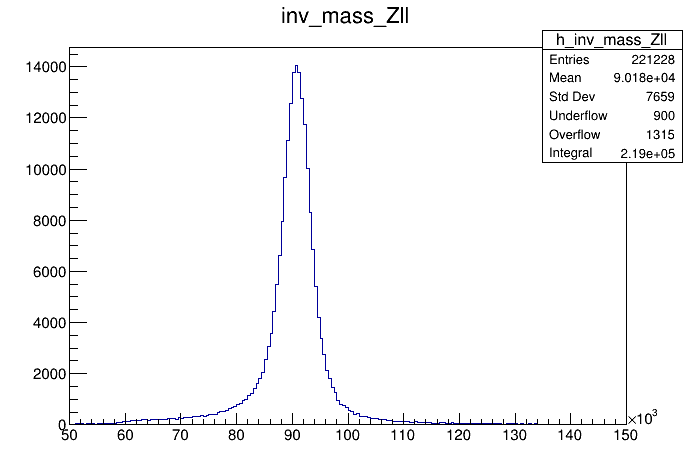
\includegraphics[width=0.85\linewidth]{plots/11-02-2021/Zll-fast_inv-mass_50-150GeV_11-02-21_11:12.png}
	\caption{(Exercise 6.4) (Fast) Plot of $Z \rightarrow ll$ invariant mass using MC data. From MC: Mean = (9.018±0.766)e+4 MeV. Expected: (9.1187±0.00021)e+4 MeV.  Cuts: 
	}
	\label{fig:zll_inv-mass_50-150GeV_11-02-21_11:12}
\end{figure}
 

\subsubsection*{\textbf{11:50} - Lead BG}
Notes/thoughts: 
\begin{itemize}
    \item larger tail towards smaller values of invaraint mass
\end{itemize}

\subsubsection*{12:00 - Exercise 6.4 - 2lep invariant mass}
Plotting the invariant mass of the 2 lepton system for the \textit{2lep} ATLAS data. S
\\
Need to specify the lepton type in the cuts.
\\
Cuts used in Fig.\ref{}:
\begin{lstlisting}

\end{lstlisting}
\begin{figure}[h!]
    \centering
	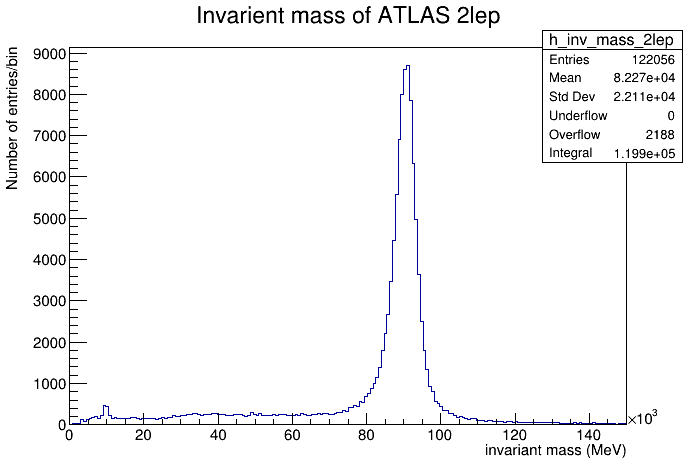
\includegraphics[width=0.85\linewidth]{plots/11-02-2021/2lep-fast_no-cuts_inv-mass_0-150GeV_11-02-21.png}
	\caption{(Exercise 6.4) (Fast) Plot of $Z \rightarrow ll$ invariant mass using MC data. From MC: Mean = (9.018±0.766)e+4 MeV. Expected: (9.1187±0.00021)e+4 MeV.  Cuts: just 2 leptons}
	\label{fig:zll_inv-mass_50-150GeV_11-02-21_11:12}
\end{figure}

\subsubsection*{\textbf{13:00}}
Break for lunch

\subsubsection*{\textbf{14:00} - Lead DG}
Working on exercise 6.7:\\
Plot graphs of ptcone30 and etcone20 for leptons that are same flavour, oppositely charged. (Zee, Zmumu, 2lep)

ptcone30 = scalar sum of track $p_T$ in a cone of R=0.3\\

Create new function 'Ptcones' in "Analysis.py" to plot the Ptcone30 of a specific lepton.

\subsubsection*{\textbf{15:10}}
To start plot ptcone30[0]:
\\
First plot - figure.\ref{fig:ptcone30_Zee_0-4GeV} of large range (0-4 GeV).\\
Data point at 0 GeV then a gap in data to 1 GeV due to. an artifact of the data of 0 - 1 GeV not being detected. \\
Would have expected an exponential decay.

\begin{figure}[h!]
    \centering
	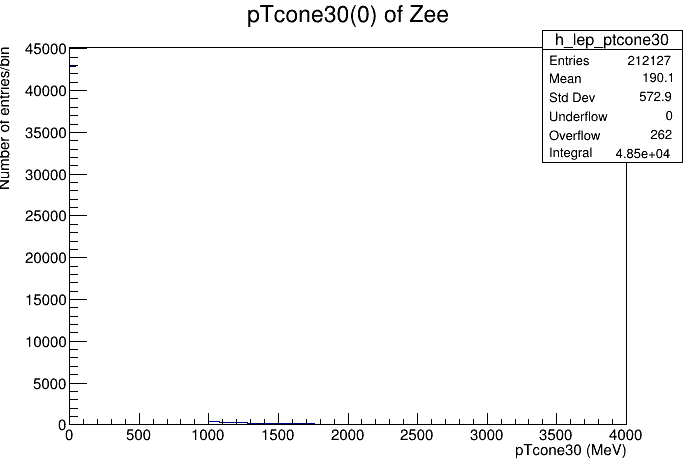
\includegraphics[width=\linewidth]{plots/11-02-2021/Zee-fast_pTcone30(0)_ 0-4Gev_11-02-2021.png}
	\caption{Plot of $Z \rightarrow ll$ pTcone30(0) using MC data. 
	}\label{fig:ptcone30_Zee_0-4GeV}
\end{figure}


\subsubsection*{\textbf{16:00} - Lead BG}

\subsubsection*{\textbf{16:11}}
Question:\\
Why is there not lep\_type = tau??
Plotting the \textbf{invariant mass} of ATLAS experimental data for at least 2 leptons with cuts to select for individual decay paths over energy range 0-150 GeV
\begin{itemize}
    \item $Z \rightarrow ee$ (lep\_type = 11 \&\& 2 particles opposite charge)
    \item $Z \rightarrow \mu\mu$ (lep\_type = 13 \&\& 2 particles opposite charge)
    \item $Z \rightarrow \tau\tau$ (Non ee and non $\tau\tau$)
\end{itemize}

Running e-e pair which is oppositely charged. Figure.\ref{fig:2lep_ee-pair_0-140GeV_11-02-21_16-12} 

\begin{figure}[h!]
    \centering
	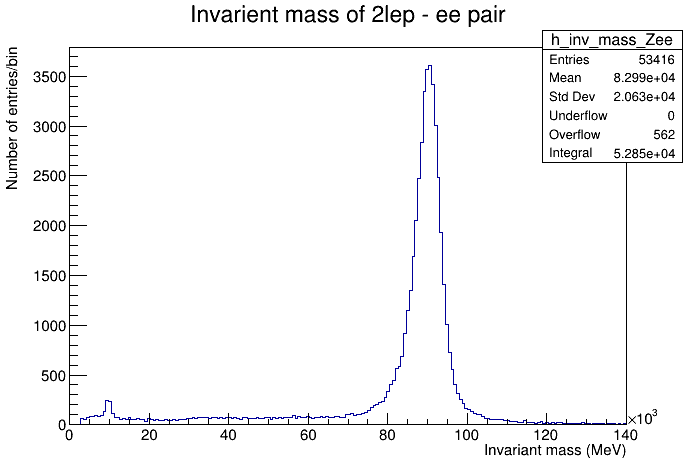
\includegraphics[width=\linewidth]{plots/11-02-2021/2lep-fast_ee-pair_inv-mass_0-140GeV_11-02-21_16-12.png}
	\caption{Plot of $Z \rightarrow ll$ pTcone30 using MC data. 
	}\label{fig:2lep_ee-pair_0-140GeV_11-02-21_16-12}
\end{figure}

Running mu-mu pair which is oppositely charged

Running non e-e and non mu-mu pair which is oppositely charged 
 returned plot no tau-tau pairs with opposite charge 
 

%%%%%%%%%%%%%% 16/02/2020 %%%%%%%%%%%%%%%%
    \newpage
    %! Author = ben
%! Date = 16/02/2021


%%%%%%%%%%%%%% 16/02/2020 %%%%%%%%%%%%%%%%
\subsection*{\textbf{16/02/2020}}
%%%%%%%%%%%%% 9:00 %%%%%%%%%%%%%
\subsubsection*{\textbf{09:00}}
Discussion of plan for the day:
\begin{itemize}
    \item Finish plotting $Z \rightarrow ll$ plots
    \item Apply cuts to pTCone30 plots
    \item etCone20 plots
\end{itemize}

%%%%%%%%%%%%% 09:23 %%%%%%%%%%%%%
\subsubsection*{09:23 - Lead DG}
Plot etcone20 to investigate what data is available.
\\
Figure.\ref{fig:Zee-fast_ETcone20(0)_0-15GeV_16-02-21_09-34}


plots Fig.\ref{fig:Zee-fast_ETcone20(1)_0-15GeV_16-02-21_09-41} of the etcone20(1)

\\
Both fig.\ref{fig:Zee-fast_ETcone20(0)_0-15GeV_16-02-21_09-34} and fig.\ref{fig:Zee-fast_ETcone20(1)_0-15GeV_16-02-21_09-41} are similar with a larger mean value for fig.\ref{fig:Zee-fast_ETcone20(1)_0-15GeV_16-02-21_09-41}.
\\
Noticed a "bump" at around 4 GeV.
\\
Plan to plot the log of the data to investigate if decay is related to exponential decay.
\begin{figure}[h!]
    \centering
    \begin{minipage}{0.5\textwidth}
        \centering
        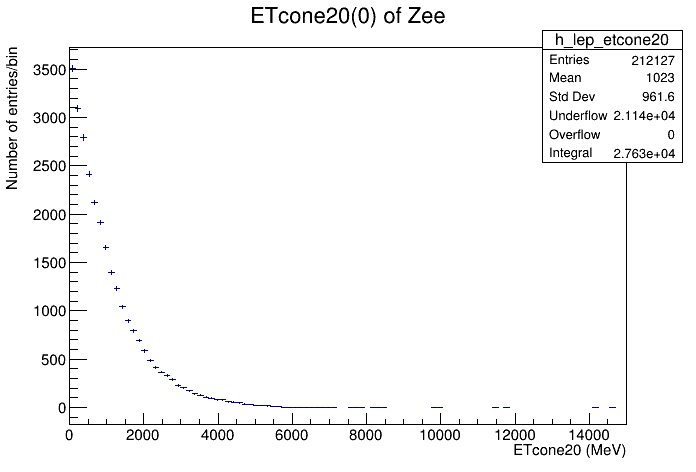
\includegraphics[width=\linewidth]{plots/16-02-2021/Zee-fast_ETcone20(0)_0-15GeV_16-02-21_09-34}
        (A)
    \end{minipage}\hfill
    \begin{minipage}{0.5\textwidth}
        \centering
        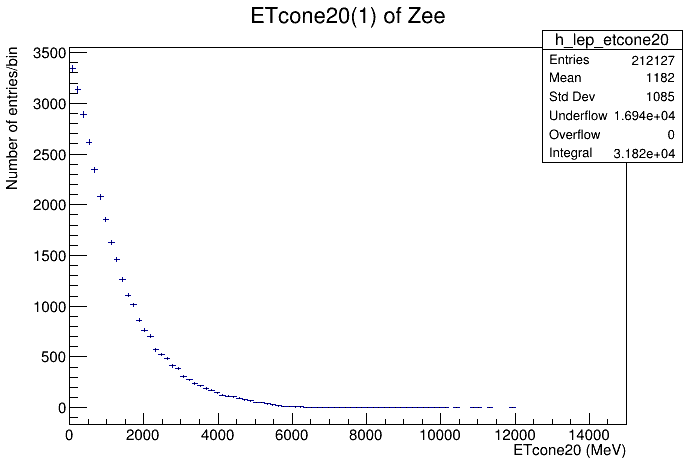
\includegraphics[width=\linewidth]{plots/16-02-2021/Zee-fast_ETcone20(1)_0-15GeV_16-02-21_09-41}
        (B)
    \end{minipage}
    \caption{ (A) Plot of $Z \rightarrow ee$ ETCone20(0) for Zee-fast MC data. (B) Plot of  $Z \rightarrow ee$ ETCone20(1) for Zee-fast MC data.}
    \label{fig:}
\end{figure}

%%%%%%%%%%%%% 09:53 %%%%%%%%%%%%%
\subsubsection*{09:53}
Plotting the ETCone of each of the two leptons produced from the decay of $Z \rightarrow \mu \mu$ using the MC data.
\begin{figure}[h!]
    \centering
    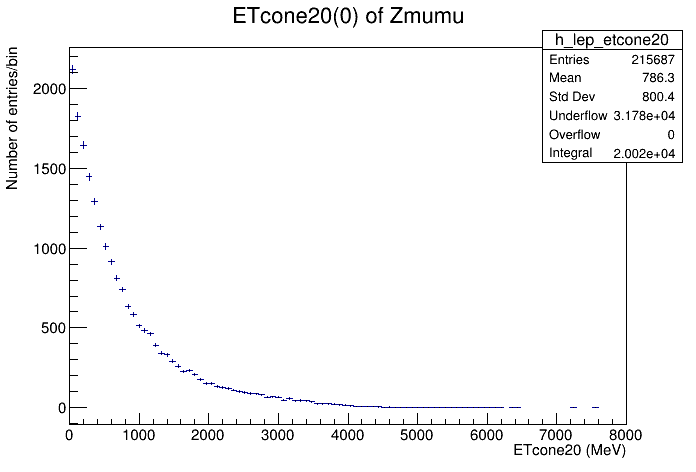
\includegraphics[width=0.85\linewidth]{plots/16-02-2021/Zmumu-fast_ETcone(0)_0-8GeV_16-02-21_09-54.png}
    \caption{Plot of  $Z \rightarrow \mu\mu$ ETCone20(0) for $Z\mu\mu$-fast MC.  data.}\label{fig:Zmumu-fast_ETcone(0)_0-8GeV_16-02-21_09-54}
\end{figure}
On fig\ref{fig:Zmumu-fast_ETcone(0)_0-8GeV_16-02-21_09-54} a slight "bump" at around 1.9 GeV

\begin{figure}[h!]
    \centering
    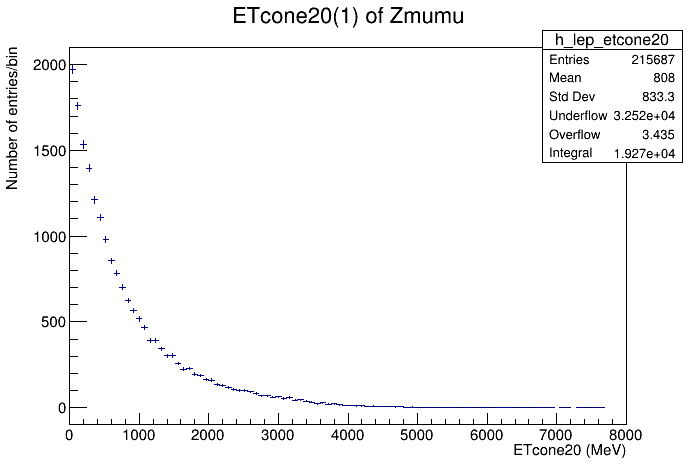
\includegraphics[width=0.85\linewidth]{plots/16-02-2021/Zmumu-fast_ETcone(1)_0-8GeV_16-02-21_09-56.png}
    \caption{Plot of  $Z \rightarrow \mu\mu$ ETCone20(1) for $Z\mu\mu$-fast MC.  data.}\label{fig:Zmumu-fast_ETcone(1)_0-8GeV_16-02-21_09-56}
\end{figure}
On fig.\ref{fig:Zmumu-fast_ETcone(1)_0-8GeV_16-02-21_09-56} the

%%%%%%%%%%%%% 10:07 %%%%%%%%%%%%%
\subsubsection*{10:07}
Plotting the pTCone30 (0)\&(1) of $Z\rightarrow ee$ for the range of 1-4 GeV. This range is used due to 0-1 GeV not being detected. (See 11-02-2021 for the investigation and plots of the full energy range.)

\begin{figure}[h!]
    \centering
    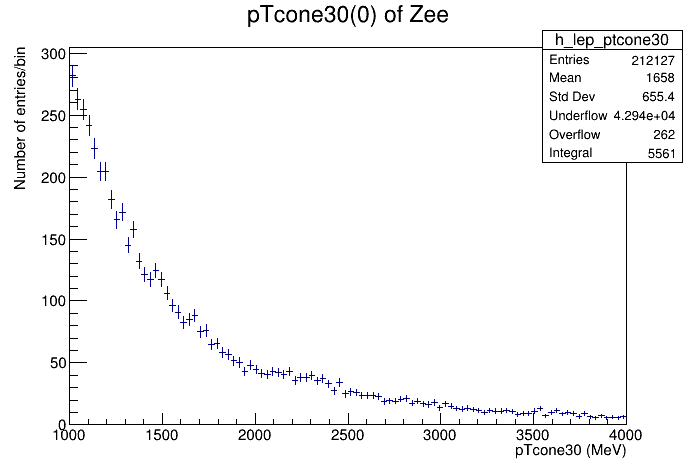
\includegraphics[width=0.85\linewidth]{plots/16-02-2021/Zee_fast_pTcone30(0)_1-4GeV_16-02-21_10-07.png}
    \caption{Plot of  $Z \rightarrow \mu\mu$ pTcone30(0) for $Z\rightarrow ee$-fast MC.  data.}\label{fig:/Zee_fast_pTcone30(0)_1-4GeV_16-02-21_10-07}
\end{figure}

On fig.\ref{fig:/Zee_fast_pTcone30(0)_1-4GeV_16-02-21_10-07}, the number of entries decrease exponentially as momentum increases.  There is also a "bump" around pTcone30 = 2.25GeV

\begin{figure}[h!]
    \centering
    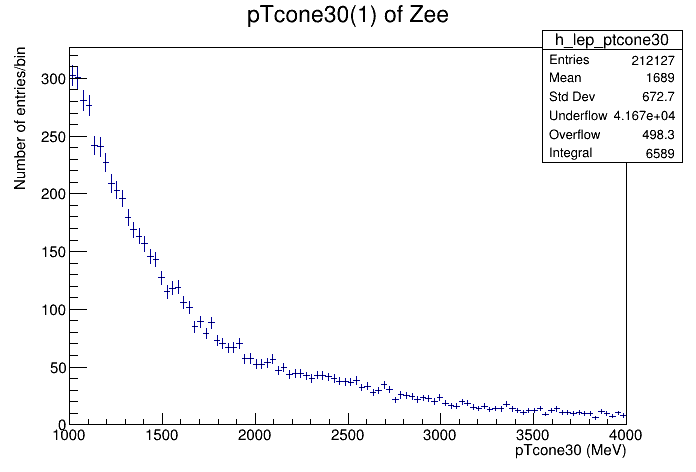
\includegraphics[width=0.85\linewidth]{plots/16-02-2021/Zee_fast_pTcone30(1)_1-4GeV_16-02-21_10-12.png}
    \caption{Plot of  $Z \rightarrow \mu\mu$ pTcone30(1) for $Z\rightarrow ee$-fast MC.  data.}\label{fig:Zee_fast_pTcone30(1)_1-4GeV_16-02-21_10-12}
\end{figure}

In fig.\ref{fig:Zee_fast_pTcone30(1)_1-4GeV_16-02-21_10-12} to "bump" seen is not as pronounced as in fig.\ref{fig:/Zee_fast_pTcone30(0)_1-4GeV_16-02-21_10-07}.


%%%%%%%%%%%%% 10:18 %%%%%%%%%%%%%
\subsubsection*{10:18}
Plotting the pTCone30 (0)\&(1) of $Z\rightarrow \mu\mu$ for the range of 1-4 GeV. This range is used due to 0-1 GeV not being detected. (See 11-02-2021 for the investigation and plots of the full energy range.)

\begin{figure}[h!]
    \centering
    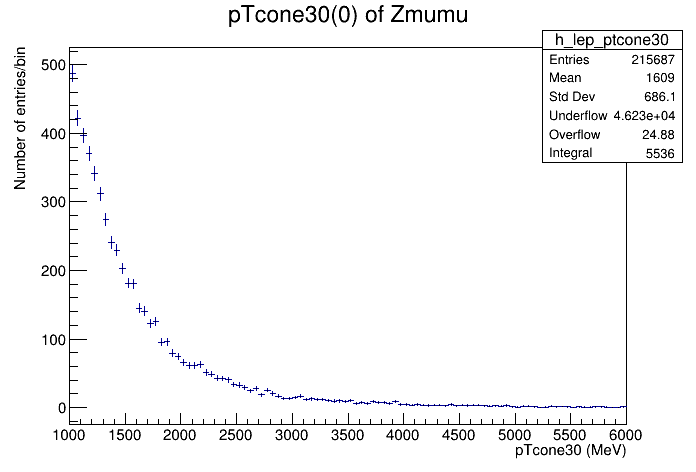
\includegraphics[width=0.85\linewidth]{plots/16-02-2021/Zmumu_fast_pTcone30(0)_1-6GeV_16-02-21_10-18.png}
    \caption{Plot of  $Z \rightarrow \mu\mu$ pTcone30(0) for $Z\mu\mu$-fast MC.  data.}\label{fig:Zmumu_fast_pTcone30(0)_1-6GeV_16-02-21_10-18}
\end{figure}

\begin{figure}[h!]
    \centering
    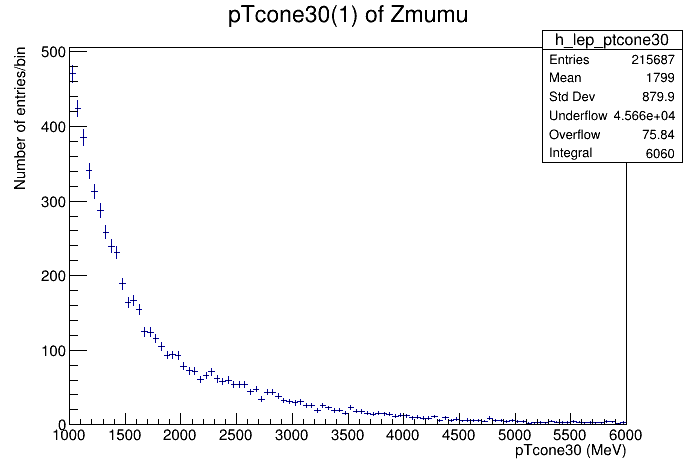
\includegraphics[width=0.85\linewidth]{plots/16-02-2021/Zmumu_fast_pTcone30(1)_1-6GeV_16-02-21_10-21.png}
    \caption{Plot of  $Z \rightarrow \mu\mu$ pTcone30(1) for $Z\mu\mu$-fast MC.  data.}\label{fig:Zmumu_fast_pTcone30(1)_1-6GeV_16-02-21_10-21}
\end{figure}


%%%%%%%%%%%%% 10:40 %%%%%%%%%%%%%
\subsubsection*{10:40}
Plotting the pTcone30 (total (sum of the two leptons)) of ATLAS data with cuts:
\begin{itemize}
    \item opposite charge
    \item lep\_type == 11 (lepton type = electron)
    \item lep\_n == 2 (number of leptons = 2)
\end{itemize}
To start, plot the range of 0-10 GeV to show 0-1 GeV is not detected.  This is seen in Fig.\ref{fig:2lep_fast_ee-pair_pTcone30(total)_0-10GeV_16-02-21_10-50} with a peak value at (total) pTcone30
\begin{figure}[h!]
    \centering
    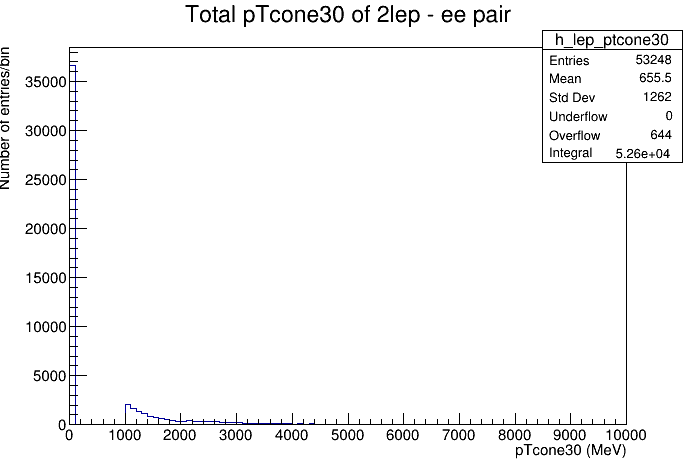
\includegraphics[width=0.85\linewidth]{plots/16-02-2021/2lep_fast_ee-pair_pTcone30(total)_0-10GeV_16-02-21_10-50}
    \caption{Plot of  $Z \rightarrow \mu\mu$ pTcone30(1) for $Z\mu\mu$-fast MC.  data.}\label{fig:2lep_fast_ee-pair_pTcone30(total)_0-10GeV_16-02-21_10-50}
\end{figure}


\begin{figure}[h!]
    \centering
    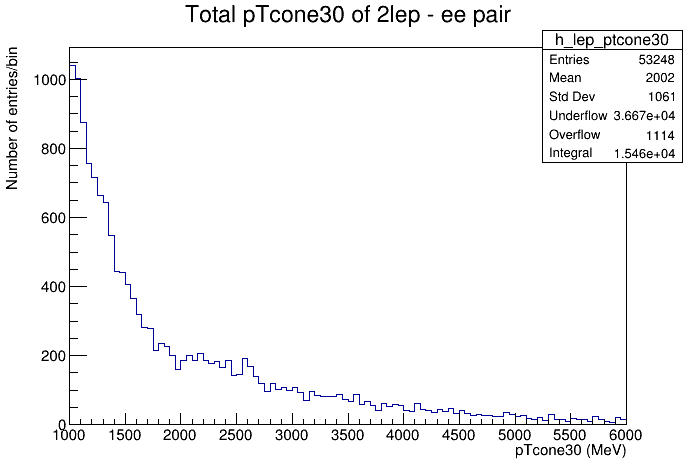
\includegraphics[width=0.85\linewidth]{plots/16-02-2021/2lep_fast_ee-pair_pTcone30(total)_1-6GeV_16-02-21_10-59}
    \caption{Plot of  $Z \rightarrow \mu\mu$ pTcone30(1) for $Z\mu\mu$-fast MC.  data.}\label{fig:2lep_fast_ee-pair_pTcone30(total)_1-6GeV_16-02-21_10-59}
\end{figure}

Fig.\ref{fig:2lep_fast_ee-pair_pTcone30(total)_1-6GeV_16-02-21_10-59} has the range set to 1-6 GeV (to remove the un-detected regoin 0-1 GeV).  This still shows exponential like decay as pTcone increases. \\
The "bump"/inconsistency (if expecting smooth exponential like decay) is present in the experiental ATLAS data around 2-2.7 GeV.  To investigate this bump, plan to plot the invariant mass with a cut to select for a pTcone30 in the vicinity of 2-2.7 GeV.

%%%%%%%%%%%%% 11:10 %%%%%%%%%%%%%
\subsubsection*{11:10}
Plotting ATLAS 2lep data for the total ETCone20 for a ee pair in the range of 0-6 GeV.  This can be seen in Fig.\ref{fig:2lep_fast_ee-pair_ETcone30(total)_0-6GeV_16-02-21_11-11}

\begin{figure}[h!]
    \centering
    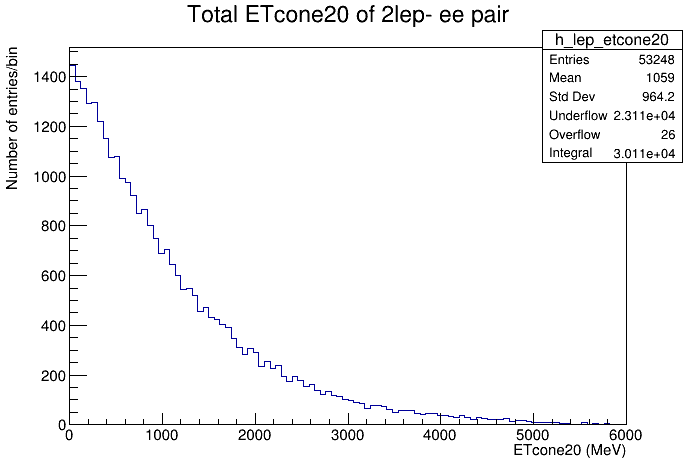
\includegraphics[width=0.85\linewidth]{plots/16-02-2021/2lep_fast_ee-pair_ETcone30(total)_0-6GeV_16-02-21_11-11}
    \caption{Plot of the total ETCone20 of an ee pair using the 2lep-fast ATLAS data.  data.}\label{fig:2lep_fast_ee-pair_ETcone30(total)_0-6GeV_16-02-21_11-11}
\end{figure}

%%%%%%%%%%%%% 11:14 %%%%%%%%%%%%%
\subsubsection*{11:14}

\begin{figure}[h!]
    \centering
    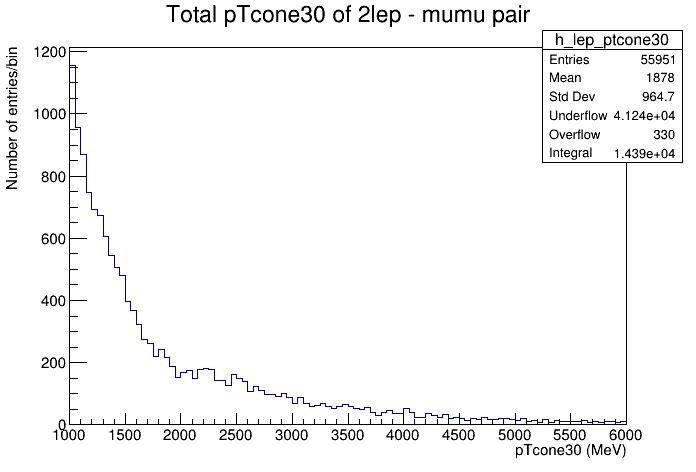
\includegraphics[width=0.85\linewidth]{plots/16-02-2021/2lep_fast_mumu-pair_pTcone30(total)_1-6GeV_16-02-21_11-06}
    \caption{Plot of the total pTcone30 of a mumu pair using the 2lep-fast ATLAS data. }\label{fig:2lep_fast_mumu-pair_pTcone30(total)_1-6GeV_16-02-21_11-06}
\end{figure}

\begin{figure}[h!]
    \centering
    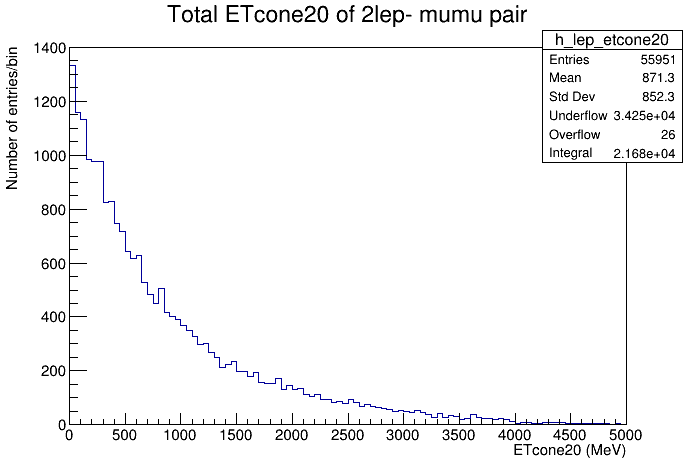
\includegraphics[width=0.85\linewidth]{plots/16-02-2021/2lep_fast_mumu-pair_ETcone30(total)_0-5GeV_16-02-21_11-14}
    \caption{Plot of the total ETcone20 of a mumu pair using the 2lep-fast ATLAS data. }\label{fig:2lep_fast_mumu-pair_ETcone30(total)_0-5GeV_16-02-21_11-14}
\end{figure}



%%%%%%%%%%%%% 11:24 %%%%%%%%%%%%%
\subsubsection*{11:24 - Lead BG}
To investigate the possible bump or dip (as seen in the pTcone30 data (bump around \dots  or dip around \dots)) plot the log of the ptCone30.


%2lep mumu logs


%pTcone
\begin{figure}[h!]
    \centering
    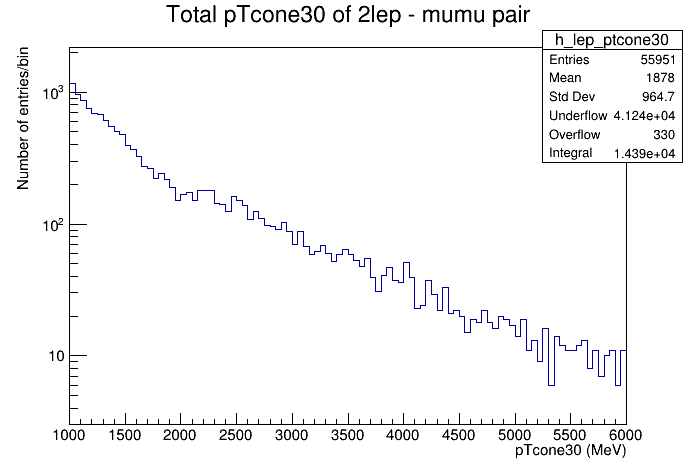
\includegraphics[width=0.85\linewidth]{plots/16-02-2021/2lep-fast_mumu_ptcone30(total)_log-entries_1-6GeV_16-02-2021_11-39}
    \caption{Plot of the total pTcone30 of a mumu pair using the 2lep-fast ATLAS data, log. }\label{fig:2lep-fast_mumu_ptcone30(total)_log-entries_1-6GeV_16-02-2021_11-39}
\end{figure}




\begin{figure}[h!]
    \centering
    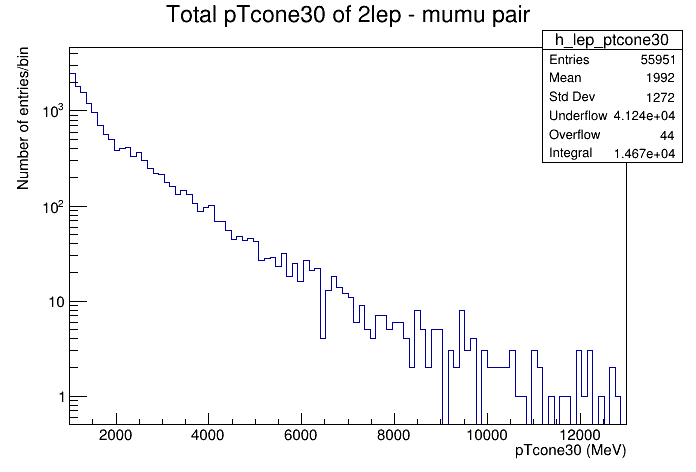
\includegraphics[width=0.85\linewidth]{plots/16-02-2021/2lep-fast_mumu-pair_ptcone30(total)_log-entries_1-13GeV_16-02-2021_11-45}
    \caption{Plot of the total pTcone30 of a mumu pair using the 2lep-fast ATLAS data, log,1-13GeV. }\label{fig:2lep-fast_mumu-pair_ptcone30(total)_log-entries_1-13GeV_16-02-2021_11-45}
\end{figure}

\begin{figure}[h!]
    \centering
    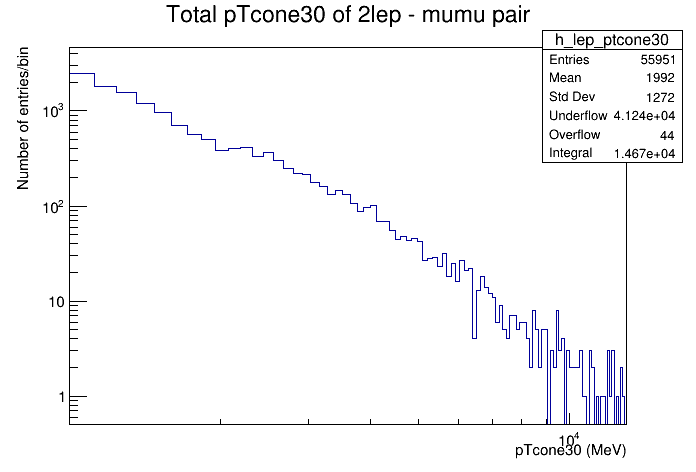
\includegraphics[width=0.85\linewidth]{plots/16-02-2021/2lep-fast_mumu-pair_ptcone30(total)_log-log_1-13GeV_16-02-2021_11-45}
    \caption{Plot of the total pTcone30 of a mumu pair using the 2lep-fast ATLAS data, log-log,1-13GeV. }\label{fig:2lep-fast_mumu-pair_ptcone30(total)_log-log_1-13GeV_16-02-2021_11-45.png}
\end{figure}


%ETcone
\begin{figure}[h!]
    \centering
    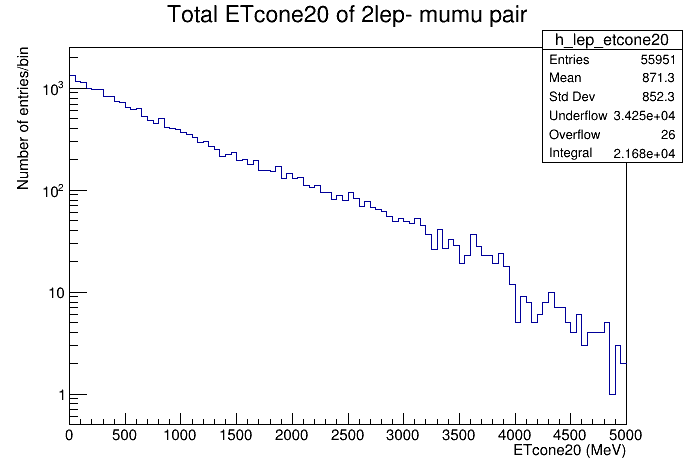
\includegraphics[width=0.85\linewidth]{plots/16-02-2021/2lep-fast_mumu-pair_etcone20(total)_log-entries_0-5GeV_16-02-2021_11-31}
    \caption{Plot of the total ETcone20 of a mumu pair using the 2lep-fast ATLAS data, log, 0-5GeV. }\label{fig:2lep-fast_mumu-pair_etcone20(total)_log-entries_0-5GeV_16-02-2021_11-31}
\end{figure}

\begin{figure}[h!]
    \centering
    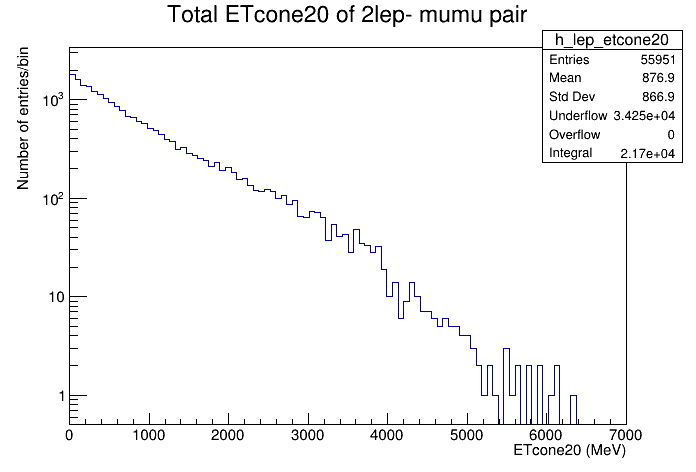
\includegraphics[width=0.85\linewidth]{plots/16-02-2021/2lep-fast_mumu-pair_etcone20(total)_log-entries_0-7GeV_16-02-2021_11-33.png}
    \caption{Plot of the total ETcone20 of a mumu pair using the 2lep-fast ATLAS data, log,0-7GeV. }\label{fig:2lep-fast_mumu-pair_etcone20(total)_log-entries_0-7GeV_16-02-2021_11-33}
\end{figure}

\subsection*{14:06- BG lead}\\
Investigate use of stacked MC plots to identify background when comparing to ATLAS data.//

\subsection*{14:50}\\
Stacked plot made for invariant. mass

\subsubsection*{16:20}
Stacked plot made for mean etcone20, includes
\begin{itemize}
    \item 2lep data
    \item Zee MC
    \item Zmumu MC
    \item Ztautau MC
\end{itemize}

\begin{figure}[h!]
    \centering
    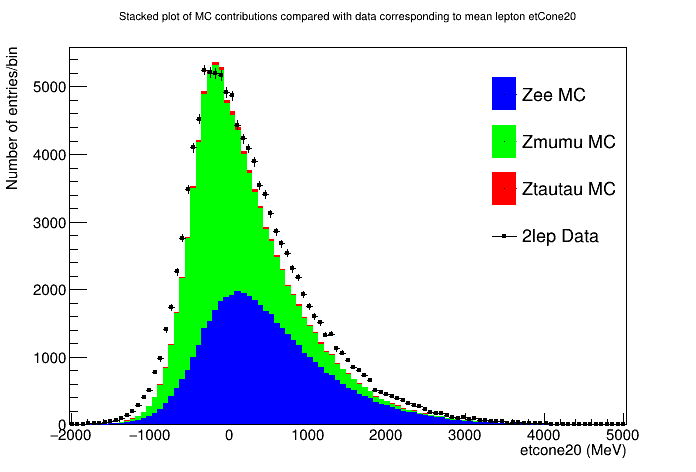
\includegraphics[width=0.85\linewidth]{plots/16-02-2021/2lep-Zee-Zmumu-Ztautau-fast_mean-etcone20_-2-5GeV_16-02-21_16-28}
    \caption{Stack plot of the mean ETcone20 of 2 lep with opposite charge pair using the 2lep-fast ATLAS data, log,0-7GeV. }\label{fig:2lep-Zee-Zmumu-Ztautau-fast_mean-etcone20_-2-5GeV_16-02-21_16-28}
\end{figure}


\subsubsection*{16:28}
Unexplained discrepancy of 2lep data around peak ~$0$MeV (Fig.\ref{fig:2lep-Zee-Zmumu-Ztautau-fast_mean-etcone20_-2-5GeV_16-02-21_16-28})

%%%%%%%%%%%%%% 18/02/2020 %%%%%%%%%%%%%%%%
    \newpage
    %%%%%%%%%%%%%% 18/02/2020 %%%%%%%%%%%%%%%% 
\subsection*{\textbf{18/02/2020}}
\subsubsection*{Days Aim}
\begin{itemize}
    \item Start to look at cross section
\end{itemize}

\subsubsection*{Day Summary}
\begin{itemize}
    \item Investigated background contributions from $ttbar_lep$, $Wplus_2lep$, and $Wminus_2lep$
    \item Calculated a preliminary value for $\sigma (Z \rightarrow ee)$ to be
    \subitem $\sigma (Z \rightarrow ee) = 1.943 nb$
\end{itemize}
%%%%%%%%%%%%% 9:00 %%%%%%%%%%%%%
\subsubsection*{09:00 - Lead BG}
Integrated Luminosity = $139 \text{fb}^{-1} (\pm 1.7\%)$

Coeficient $\epsilon$ given by sum of MC signal weights over that for relevent sample (found using TotExpected.Py) 

Made stacked plots for pTcone30 and etcone. Unexplained discrepancy of 2lep data aorund peak ~$0$MeV (Figure \ref{fig:2lep-Zee-Zmumu-Ztautau-fast_mean-etcone20_-2-5GeV_16-02-21_16-28}) 


Add ttbar\_lep to stack plots


$\epsilon_{\text{Zee}}$ = 19630128.89 

Quoted value for Zee cross section $76.0 \pm 0.8 \pm 2.0 \pm 2.6$ pb (https://arxiv.org/pdf/1212.4620.pdf)

%%%%%%%%%%%%% 10:38 %%%%%%%%%%%%%
\subsubsection*{10:38}

Rough estimate for the cross section: $\sigma (pp \rightarrow Z \rightarrow ee)$ is given by:
\begin{align}
    \sigma &= \frac{N^{selected} - N^{background}}{\epsilon \int L dt}
\end{align}
where
\begin{align}
     \epsilon &= \frac{\sum \text{weights for all MC events which pass selection cuts}}{\sum \text{weights for all events for that process}} 
\end{align}
For $Z \rightarrow ee$ use the cuts:
\begin{itemize}
    \item lep\_n = 2
    \item same flavour/type (lep\_type [0] == lep\_type[1])
    \item opposite charge (lep\_charge [0] != lep\_charge[1])
    \item invariant mass > 60 GeV 
    \subitem MC not modelled below this point
\end{itemize}
For $\sigma (pp \rightarrow Z \rightarrow ee)$:
\begin{itemize}
    \item $N^{selected} = 47531$
    \item $N^{background} = 0$
    \item $\epsilon = \frac{46740}{19630128.89} = $
    \item $\int L dt = 10.064 \textbf{fb}^{-1}$
\end{itemize}


cs = 1.9835391029941325e-09
\\
Other sources of background 
 - photon conversion 
 - hadronic jets
 -W or t decays can be detected as 2 electrons or muons when one is in fact a hadron jet or electron/moun from other source. 
 
%%%%%%%%%%%%% 14:00 %%%%%%%%%%%%%
\subsubsection*{14:00 - Lead DG - Number of leptons from W-plus and W-minus}
Investigating the decay paths of W-plus and W-minus.
\\
Plotting the number of leptons per event ($lep_n$)
\\
Cuts used in Fig.\ref{fig:14-00_18-02-21}:
\begin{lstlisting}
lepCut = "(" + "(lep_charge[0] != lep_charge[1]) && (lep_type[0] == lep_type[1]) && lep_n==2" + ")"

t.Draw("lep_n >> h_lep_n(100,0,100)", weighting + "*" + lepCut)
\end{lstlisting}
\begin{figure}[h!]
    \centering
    \begin{minipage}{0.5\textwidth}
        \centering
        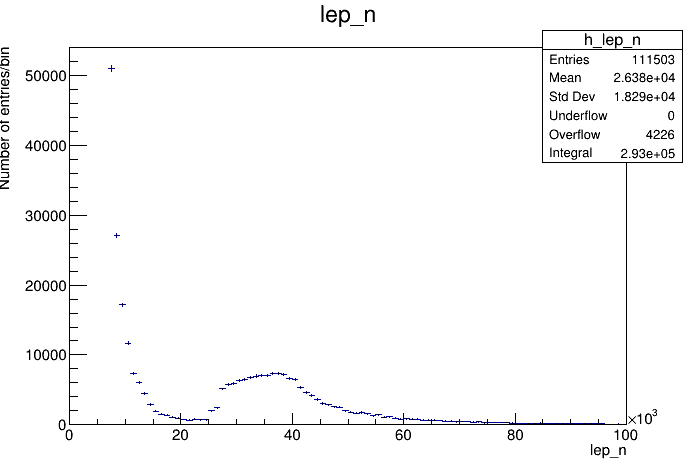
\includegraphics[width=\linewidth]{plots/18-02-2021/Wminus_2lep_lep_n_0-100_18-02-2021_14-12.png}
        (A)
    \end{minipage}\hfill
    \begin{minipage}{0.5\textwidth}
        \centering
        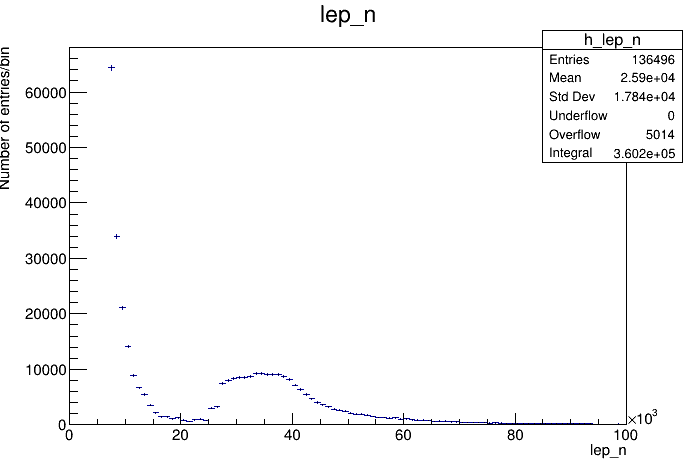
\includegraphics[width=\linewidth]{plots/18-02-2021/Wplus_2lep_slow_lep_n_0-100000_18-02-21_14-17.png}
        (B)
    \end{minipage}
    \caption{(A) Number of leptons in each event for Wminus-2lep. (B) Number of leptons in each event for Wplus-2lep. Cuts = basic: lepton pair with opposite charge and same type.}
    \label{fig:14-00_18-02-21}
\end{figure}
% (A) Wminus_2lep_lep_n_0-100_18-02-2021_14-12.png
% (B) Wplus_2lep_slow_lep_n_0-100000_18-02-21_14-17.png

There is an exponential decay in the number of leptons apart from a bump at about 35 leptons.
\\
This indicates that these leptons are most likely a result of lepton showers/jets.


%%%%%%%%%%%%% 14:40 %%%%%%%%%%%%%
\subsubsection*{14:40 - Invariant mass for Wplus-2lep and Wminus-2lep (Z -> ll)}
Plot the invariant mass between 60-150GeV for Wplus-2lep and Wminus-2lep for events that would look like $Z \rightarrow ll$.
\\
Large underflow, so increase range to 0-150 GeV 
\\
Still not totally decayed, increase range to 0-500 GeV.
\\
Cuts used in. Fig.\ref{fig:14-40_18-02-2021}:
\begin{lstlisting}
lepCut = "(" + "lep_n == 2 && (lep_charge[0] != lep_charge[1]) &&  (lep_type[0] == lep_type[1]) " + ")"

t.SetAlias("inv_mass_Zll","sqrt(2*lep_pt[0]*lep_pt[1]*(cosh(lep_eta[0]-lep_eta[1])-cos(lep_phi[0]-lep_phi[1])))")
  
t.Draw("inv_mass_Zll >> h_inv_mass(100,0,150e3)", weighting + "*" + lepCut)
\end{lstlisting}
\begin{figure}[h!]
    \centering
    \begin{minipage}{0.5\textwidth}
        \centering
        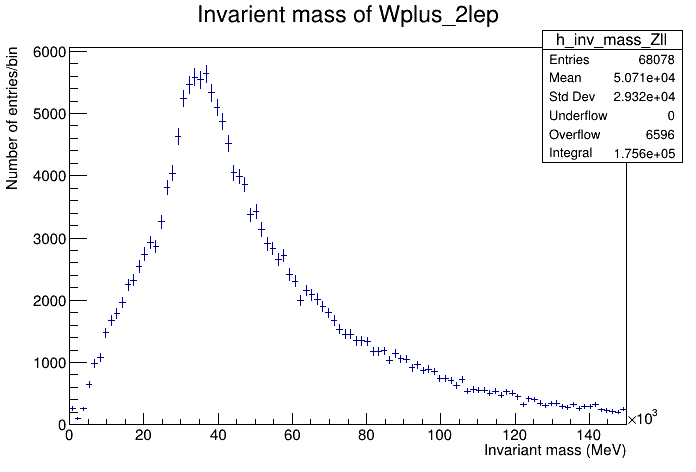
\includegraphics[width=\linewidth]{plots/18-02-2021/Invarient mass of Wplus_2lep 18-02-2021_14_49 .png}
        (A)
    \end{minipage}\hfill
    \begin{minipage}{0.5\textwidth}
        \centering
        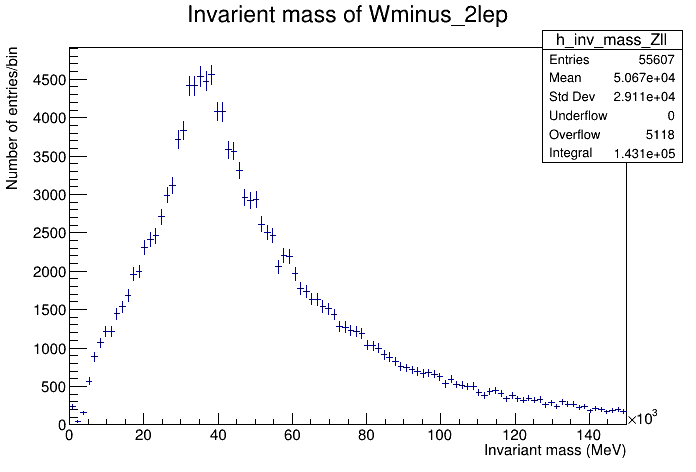
\includegraphics[width=\linewidth]{plots/18-02-2021/Wminus-2lep_invar-mass_18-02-21_14-54.png}
        (B)
    \end{minipage}
    \caption{(A) Invariant mass from Wplus-2lep (Background contribution) (B) Invariant mass from Wminus-2lep.  Cuts: (basic) lepton pair with oppsite charge and same type.}
    \label{fig:14-40_18-02-2021}
\end{figure}


%%%%%%%%%%%%% 16:10 %%%%%%%%%%%%%
\subsubsection*{16:00 - Lead BG - preliminary $\sigma (Z \rightarrow ee)$}
Finding the background contributions from $W^+ \rightarrow l\nu_l $ with the cut 
\begin{lstlisting}
     lepCut ="(" + "(lep_charge[0] != lep_charge[1]) && (lep_type[0]==11 && lep_type[1]==11) && lep_n==2 && (inv_mass_Zll > 60e3) && (inv_mass_Zll < 115e3)" + ")"
\end{lstlisting}
to select for e+e- pair.
\begin{align}
    N^{background}_{t\Bar{t}} &= 236276
    \\
    N^{background}_{W^+} &= 2247
    \\
    N^{background}_{W-} &= 1785
\end{align}
Sum of all weights for all MC events which pass cuts for Zee:
\begin{align*}
    = 4595000
\end{align*}
 
4817004

$\sigma(Z \rightarrow ee) = 1.94275964340403e-09 b$

//
TODO: 
\begin{itemize}
    \item Plot $ \Delta \phi$ 
    \item $\epsilon$ cut
\end{itemize}





%%%%%%%%%%%%%% 23/02/2020 %%%%%%%%%%%%%%%%
    \newpage
    %%%%%%%%%%%%%% 23/02/2020 %%%%%%%%%%%%%%%% 
\subsection*{\textbf{23/02/2020}}

\subsubsection*{Days aims}
\begin{itemize}
    \item Investigate $\Delta \phi$
    \item 
\end{itemize}

\subsubsection*{Day Summary}
\begin{itemize}
    \item Investigated $\Delta \phi$
    \item Applied ptcone30 cut to invariant mass
    \item Plotted etcone20 with ptcone30 cuts
    
    \item Found pT upper cut of:
    \subitem 34 GeV for mumu 
    \subitem 36 GeV for ee 
    
    \item Plotted $\eta$ - ruled out as a cut
    
    \item 
\end{itemize}
%%%%%%%%%%%%% 9:00 %%%%%%%%%%%%%
\subsubsection*{08:30 - Lead BG}
The ATLAS detector can mistake the production of a $l^+ l^-$ pair from 2 seperate decays as pair production from the decay of a single particle, such as a Z boson. 
\\
A possible source of this is from W boson decays:
\begin{align*}
    W^+ \rightarrow l^+ \nu_{l}
    \\
    W^- \rightarrow l^- \Bar{\nu_{l}}
\end{align*}
to be mistaken for $Z \rightarrow ll$.
\\
In the case of $Z \rightarrow ll$, the two leptons would be expected to be produced with the angle between them ($\Delta \phi$) $\approx \pi$ (angle between the azimuthal angle) to conserve momentum.
\\
Counter to this, the  $W^+ \rightarrow l^+ \nu_{l}$ and $W^- \rightarrow l^- \Bar{\nu_{l}}$ can be proceed at any angle, so would expect production to include $\Delta \phi \approx 0$
\\
To investigate this, plot $\Delta \phi$ of ATLAS "2lep" data, the cuts used in Fig.\ref{fig:23-02_09-43} are:
\begin{lstlisting}
lepCut ="(" + "(lep_charge[0] != lep_charge[1]) && (lep_type[0]==13 && lep_type[1]==13) && lep_n==2 && (inv_mass_Zll > 60e3)" + ")"
    
t.SetAlias("inv_mass_Zll","sqrt(2*lep_pt[0]*lep_pt[1]*(cosh(lep_eta[0]-lep_eta[1])-cos(lep_phi[0]-lep_phi[1])))")

t.Draw("abs(lep_phi[0] - lep_phi[1]) >> h_lep_delta_phi(100,0,6.3)", weighting + "*" + lepCut)
\end{lstlisting}

Fig.\ref{fig:23-02_09-43} shows that there is a small peak at loer angles.  This can be produced from. two main processes:
\begin{itemize}
    \item Momentum conservation to compensate for jets
    \item incorrect classification for two W+ and W- decays.
\end{itemize}

\begin{figure}[h!]
    \centering
    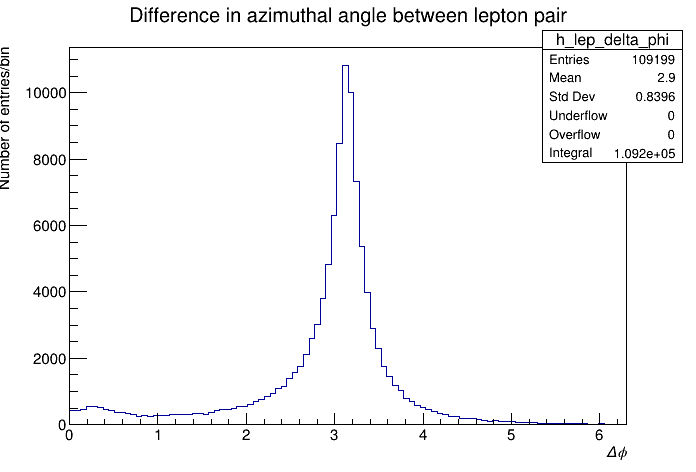
\includegraphics[width=0.85\linewidth]{plots/23-02-2021/2lep_delta-phi_0-7_23-02_09-43.png}
    \caption{The difference of the azimuthal angle of the lepton pair for the 2lep ATLAS data.  The main peak at approx $\pi$ is as expected}\label{fig:23-02_09-43}
\end{figure}

%%%%%%%%%%%%% 9:48 %%%%%%%%%%%%%
\subsubsection*{09:48 - Lead DG}
Apply ptcone20 cut on invariant mass plots.
\\
Since there is no distinction between events in the range 0-1 GeV, cut events above 1 GeV.
\\
Since variables/quantities are correlated (can be effected by the same physical process), plot the etcone20 stack plot.   See Fig.\ref{}

%%%%%%%%%%%%% 14:07 %%%%%%%%%%%%%
\subsubsection*{14:07 - Lead BG}
Plot pT log to test for potential cuts.

Test other kinematic variables to look for potential cuts

Upper bound cut of 320GeV for total lepton pair pT.  See Fig.{}

%%%%%%%%%%%%% 15:24 %%%%%%%%%%%%%
\subsubsection*{15:24 - Lead DG - Plot $\eta$}
Plot eta in search of potential cuts. 
\\
Cuts used for Fig.\ref{fig:15-24_23-02-21}:
\begin{lstlisting}
lepCut ="(" + "(lep_charge[0] != lep_charge[1]) && (lep_type[0]==lep_type[1]) && lep_n==2" + ")"
    
t.Draw("abs(lep_eta[0]) >> h_lep_eta(100,0,3)", weighting + "*" + lepCut)
\end{lstlisting}
\begin{figure}[h!]
    \centering
	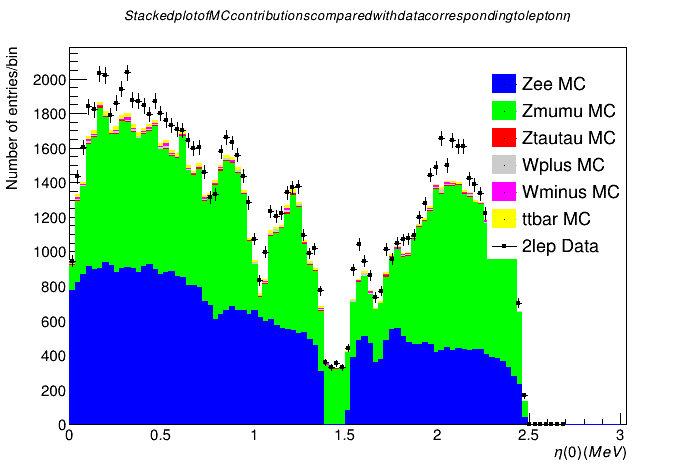
\includegraphics[width=0.85\linewidth]{plots/23-02-2021/All-stack-fast_eta_0-3_.png}
	\caption{Stack plot for the absolute value of $eta$ for lepton [0] to include signal and and background 2lep and MC.  Cuts: lepton pair of same flavour/type and opposite charge. }\label{fig:15-24_23-02-21}
\end{figure}


%%%%%%%%%%%%% 15:31 %%%%%%%%%%%%%
\subsubsection*{15:31}
Plot the stack plot of delta phi in search of possible cuts.
\\
First apply only minimal cuts (no lower from invariant mass and upper ):
\begin{lstlisting}
lepCut ="(" + "(lep_charge[0] != lep_charge[1]) && (lep_type[0]==13 && lep_type[1]==13) && lep_n==2 && (inv_mass_Zll > 60e3)" + ")"
    
t.SetAlias("inv_mass_Zll","sqrt(2*lep_pt[0]*lep_pt[1]*(cosh(lep_eta[0]-lep_eta[1])-cos(lep_phi[0]-lep_phi[1])))")

t.Draw("abs(lep_phi[0] - lep_phi[1]) >> h_lep_delta_phi(100,0,6.3)", weighting + "*" + lepCut)
\end{lstlisting}
\begin{figure}[h!]
    \centering
	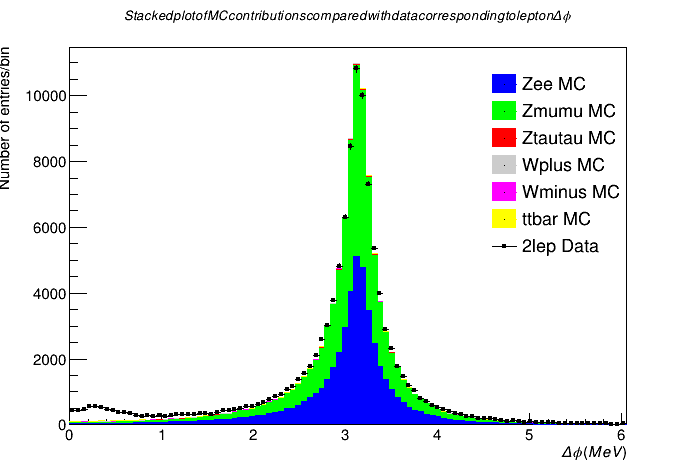
\includegraphics[width=0.85\linewidth]{plots/23-02-2021/All-stack-fast_delta-phi_minimal-cuts_0-6_23-02-21_15-30.png}
	\caption{Stack plot of delta phi with only minimal cuts to select for events with 2 leptons of same type with opposite charge.  There is an inconstancy between MC and ATLAS data (\textbf{NOT MeV - should be rad})}\label{fig:All-stack-fast_delta-phi_minimal-cuts_0-6_23-02-21_15-30}
\end{figure}
From Fig.\ref{fig:All-stack-fast_delta-phi_minimal-cuts_0-6_23-02-21_15-30}:
- Inconstancy between MC and ATLAS data around 0-1 rad.

Now add upper from total transverse momentum and lower from invariant mass.
\begin{figure}[h!]
    \centering
	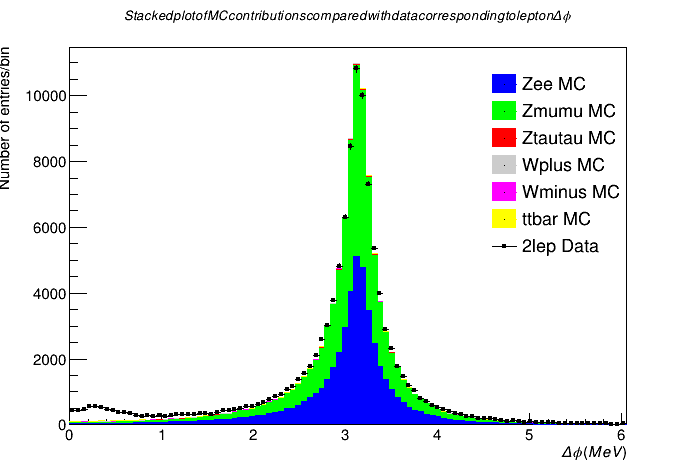
\includegraphics[width=0.85\linewidth]{plots/23-02-2021/All-stack-fast_delta-phi_minimal-cuts_0-6_23-02-21_15-30.png}
	\caption{Stack plot of delta phi with only minimal cuts to select for events with 2 leptons of same type with opposite charge.  There is an inconsitancy between MC and ATLAS for $\Delta \phi < 1 rad$ (\textbf{NOT MeV - should be rad})}\label{fig:All-stack-fast_delta-phi_minimal-cuts_0-6_23-02-21_15-30}
\end{figure}
From Fig.\ref{}:
-> Good MC fit to ATLAS data - no more "bump" between 0-1 rad

Question: Is it better to make cuts based on individual particles or total/mean.
 
 %%%%%%%%%%%%% 15:54 %%%%%%%%%%%%%
\subsubsection*{15:54 - Lead BG}
Start to calculate the cross section of $pp \rightarrow Z \rightarrow ee$ with the new cuts (lower and upper bounds on variables).
\\
Cuts being used:
\begin{lstlisting}
lepCut ="(" + "(lep_charge[0] != lep_charge[1]) && (lep_type[0]==lep_type[1]) && lep_n==2 && (inv_mass_Zll > 60e3) && (lep_pt[0]+lep_pt[1]) < 320e3 " + ")"
\end{lstlisting}

%%%%%%%%%%%%% 17:00 %%%%%%%%%%%%%
\subsubsection*{17:00 - Logout}

\end{document}